% 注意事项:编译两次,以确保目录、页码完整显示

\def\allfiles{}

\documentclass[14pt,a4paper,UTF8,twoside]{article}

% Formatting Packages ——————————————————————————————————————
\usepackage{multicol}
\usepackage{multirow}
\usepackage{enumitem}
\usepackage{indentfirst}
\usepackage[toc]{multitoc}

% Math & Physics Packages ————————————————————————————
\usepackage{amsmath, amsthm, amsfonts, amssymb}
\usepackage{setspace}
\usepackage{physics}
\usepackage{cancel}
\usepackage{nicefrac}
\usepackage{unicode-math} % 允许数学公式使用特定字体

% Image-related Packages —————————————————————————————
\usepackage{float} % 浮动体环境
\usepackage{subcaption} % 子图包
\usepackage{graphics, graphicx}
\usepackage{tikz, tikz-qtree}
\usetikzlibrary{arrows.meta}
\usepackage{pgfplots}
\pgfplotsset{compat=1.18}
\usepackage{xcolor}
\usepackage{fourier-orns}
\usepackage{lipsum}

% Colour Palette ——————————————————————————————————————
\definecolor{merah}{HTML}{F4564E}
\definecolor{merahtua}{HTML}{89313E}
\definecolor{biru}{HTML}{60BBE5}
\definecolor{birutua}{HTML}{412F66}
\definecolor{hijau}{HTML}{59CC78}
\definecolor{hijautua}{HTML}{366D5B}
\definecolor{kuning}{HTML}{FFD56B}
\definecolor{jingga}{HTML}{FBA15F}
\definecolor{ungu}{HTML}{8C5FBF}
\definecolor{lavender}{HTML}{CBA5E8}
\definecolor{merjamb}{HTML}{FFB6E0}
\definecolor{mygray}{HTML}{E6E6E6}
\definecolor{mygreen}{rgb}{0,0.6,0}
\definecolor{mymauve}{rgb}{0.58,0,0.82}

% Theorems ————————————————————————————————————————————
\usepackage{tcolorbox}
\usepackage{changepage}
\tcbuselibrary{skins,breakable,theorems}

\newcounter{hitung}
\setcounter{hitung}{\thesection}

\makeatletter
	% Proof 证明如下
	\def\tcb@theo@widetitle#1#2#3{\hbox to \textwidth{\textsc{\large#1}\normalsize\space#3\hfil(#2)}}
	\tcbset{
		theorem style/theorem wide name and number/.code={ \let\tcb@theo@title=\tcb@theo@widetitle},
		proofbox/.style={skin=enhancedmiddle,breakable,parbox=false,boxrule=0mm,
			check odd page, toggle left and right, colframe=black!20!white!92!hijau,
			leftrule=8pt, rightrule=0mm, boxsep=0mm,arc=0mm, outer arc=0mm,
			left=3mm,right=3mm,top=0mm,bottom=0mm, toptitle=0mm,
			bottomtitle=0mm,colback=gray!3!white!98!biru, before skip=8pt, after skip=8pt,
			before={\par\vskip-2pt},after={\par\smallbreak},
		},
	}
	\newtcolorbox{ProofBox}{proofbox}
	\makeatother
	
	\let\realproof\proof
	\let\realendproof\endproof
	\renewenvironment{proof}[1][Prove:]{\ProofBox\strut\textsc{#1}\space}{\endProofBox}
        \AtEndEnvironment{proof}{\null\hfill$\blacksquare$}
        % Definition 定义环境
	\newtcbtheorem[use counter=hitung, number within=section]{dfn}{定义}
	{theorem style=theorem wide name and number,breakable,enhanced,arc=3.5mm,outer arc=3.5mm,
		boxrule=0pt,toprule=1pt,leftrule=0pt,bottomrule=1pt, rightrule=0pt,left=0.2cm,right=0.2cm,
		titlerule=0.5em,toptitle=0.1cm,bottomtitle=-0.1cm,top=0.2cm,
		colframe=white!10!biru,
		colback=white!90!biru,
		coltitle=white,
		shadow={1.3mm}{-1.3mm}{0mm}{gray!50!white}, % 添加阴影
        coltext=birutua!60!gray, title style={white!10!biru}, rbefoe skip=8pt, after skip=8pt,
		fonttitle=\bfseries,fontupper=\normalsize}{dfn}

	% 答题卡
	\newtcbtheorem[use counter=hitung, number within=section]{ans}{解答}
	{theorem style=theorem wide name and number,breakable,enhanced,arc=3.5mm,outer arc=3.5mm,
		boxrule=0pt,toprule=1pt,leftrule=0pt,bottomrule=1pt, rightrule=0pt,left=0.2cm,right=0.2cm,
		titlerule=0.5em,toptitle=0.1cm,bottomtitle=-0.1cm,top=0.2cm,
		colframe=white!10!biru,
		colback=white!90!biru,
		coltitle=white,
		shadow={1.3mm}{-1.3mm}{0mm}{gray!50!white}, % 添加阴影
        coltext=birutua!60!gray, title style={white!10!biru}, before skip=8pt, after skip=8pt,
		fonttitle=\bfseries,fontupper=\normalsize}{ans}

	% Axiom
	\newtcbtheorem[use counter=hitung, number within=section]{axm}{公理}
	{theorem style=theorem wide name and number,breakable,enhanced,arc=3.5mm,outer arc=3.5mm,
		boxrule=0pt,toprule=1pt,leftrule=0pt,bottomrule=1pt, rightrule=0pt,left=0.2cm,right=0.2cm,
		titlerule=0.5em,toptitle=0.1cm,bottomtitle=-0.1cm,top=0.2cm,
		colframe=white!10!biru,colback=white!90!biru,coltitle=white,
		shadow={1.3mm}{-1.3mm}{0mm}{gray!50!white!90}, % 添加阴影
        coltext=birutua!60!gray,title style={white!10!biru},before skip=8pt, after skip=8pt,
		fonttitle=\bfseries,fontupper=\normalsize}{axm}
 
	% Theorem
	\newtcbtheorem[use counter=hitung, number within=section]{thm}{定理}
	{theorem style=theorem wide name and number,breakable,enhanced,arc=3.5mm,outer arc=3.5mm,
		boxrule=0pt,toprule=1pt,leftrule=0pt,bottomrule=1pt, rightrule=0pt,left=0.2cm,right=0.2cm,
		titlerule=0.5em,toptitle=0.1cm,bottomtitle=-0.1cm,top=0.2cm,
		colframe=white!10!merah,colback=white!75!pink,coltitle=white, coltext=merahtua!80!merah,
		shadow={1.3mm}{-1.3mm}{0mm}{gray!50!white!90}, % 添加阴影
		title style={white!10!merah}, before skip=8pt, after skip=8pt,
		fonttitle=\bfseries,fontupper=\normalsize}{thm}
	
	% Proposition
	\newtcbtheorem[use counter=hitung, number within=section]{prp}{命题}
	{theorem style=theorem wide name and number,breakable,enhanced,arc=3.5mm,outer arc=3.5mm,
		boxrule=0pt,toprule=1pt,leftrule=0pt,bottomrule=1pt, rightrule=0pt,left=0.2cm,right=0.2cm,
		titlerule=0.5em,toptitle=0.1cm,bottomtitle=-0.1cm,top=0.2cm,
		colframe=white!10!hijau,colback=white!90!hijau,coltitle=white, coltext=hijautua!80!brown,
		shadow={1.3mm}{-1.3mm}{0mm}{gray!50!white}, % 添加阴影
		title style={white!10!hijau}, before skip=8pt, after skip=8pt,
		fonttitle=\bfseries,fontupper=\normalsize}{prp}


	% Example
	\newtcolorbox[use counter=hitung, number within=section]{cth}[1][]{breakable,
		colframe=white!10!jingga, coltitle=white!90!jingga, colback=white!85!jingga, coltext=black!10!brown!50!jingga, colbacktitle=white!10!jingga, enhanced, fonttitle=\bfseries,fontupper=\normalsize, attach boxed title to top left={yshift=-2mm}, before skip=8pt, after skip=8pt,
		title=Contoh~\thetcbcounter \ \ #1}

	% Catatan/Note
	\newtcolorbox{ctt}[1][]{enhanced, 
		left=4.1mm, borderline west={8pt}{0pt}{white!10!kuning}, 
		before skip=6pt, after skip=6pt, 
		colback=white!85!kuning, colframe= white!85!kuning, coltitle=orange!60!kuning!25!brown, coltext=orange!60!kuning!25!brown,
		fonttitle=\bfseries,fontupper=\normalsize, before skip=8pt, after skip=8pt,
		title=\underline{Catatan}  #1}
	
	% Komentar/Remark
	\newtcolorbox{rmr}[1][]{
		,arc=0mm,outer arc=0mm,
		boxrule=0pt,toprule=1pt,leftrule=0pt,bottomrule=5pt, rightrule=0pt,left=0.2cm,right=0.2cm,
		titlerule=0.5em,toptitle=0.1cm,bottomtitle=-0.1cm,top=0.2cm,
		colframe=white!10!kuning,colback=white!85!kuning,coltitle=white, coltext=orange!60!kuning,
		fonttitle=\bfseries,fontupper=\normalsize, before skip=8pt, after skip=8pt,
		title=Komentar  #1}

\usepackage{booktabs} % 表格库
\usepackage{titlesec} % 标题库
\usepackage{fancyhdr} % 页眉页脚库
\usepackage[sorting=none]{biblatex}
\usepackage{array}
\addbibresource{references.bib} % 指定你的.bib文件名称

\date{} % 留空,以让编译时去除日期

%———————————————注意事项—————————————————%

% 1、如果编译显示失败,但没有错误信息,就是 filename.pdf 正在被占用
% 2、在文件夹中的终端使用 Windows > xelatex filename.tex 也可编译

%—————————————华东师范大学———————————————%

% 论文制作时须加页眉,页眉从中文摘要开始至论文末
% 偶数页码内容为:华东师范大学硕士学位论文,奇数页码内容为学位论文题目

%————————定义 \section 的标题样式————————%

% 注意:\chapter 等命令,内部使用的是 \thispagestyle{plain} 的排版格式
% 若需要自己加上页眉,实际是在用 \thispagestyle{fancy} 的排版格式
% 加上下面这一段指令,就能够让 \section 也使用 fancy 的排版格式
% 本质就是让目录、第一页也能够显示页眉、页脚

\fancypagestyle{plain}{
  \pagestyle{fancy}
}

\title{华东师范大学软件学院课程作业} % 模板
\titleformat{\section}
    {\normalfont\bfseries\Large} % 字体大小、字体系列(\bfseries 为加粗)
    {\thesection}{1em}{}

% ———————————设置章节的中文格式———————————%
\renewcommand\thesection{\chinese{section} \hspace{0pt}}
\renewcommand\thesubsection{\arabic{subsection} \hspace{0pt}}
% \renewcommand\thesubsubsection{\alph{subsubsection} \hspace{0pt}} % 字母编号
% \hspace{0pt} 是为了确保在章节编号和章节题目之间不要有空格,使得排版更为美观
    
%—————————————页面基础设置———————————————%

\usepackage{geometry}
\geometry{left=10mm, right=10mm, top=20mm, bottom=20mm}

%————————————设置页眉、页脚——————————————%

\pagestyle{fancy} % 设置 plain style 的属性

% 设置页眉

\fancyhead[RE]{\footnotesize \leftmark} % Right Even 偶数页右侧显示章名 \leftmark 最高级别章名
\fancyhead[LO]{\footnotesize \rightmark} % Left Odd 奇数页左侧显示节名 \rightmark 第二级别节名
\fancyhead[C]{华东师范大学软件学院课程作业} % Center 居中显示
\fancyhead[LE,RO]{~\thepage~} % 在偶数页的左侧,奇数页的右侧显示页码
\renewcommand{\headrulewidth}{1.2pt} % 页眉与正文之间的水平线粗细

% 设置页脚:在每页的右下脚以斜体显示书名

\fancyfoot[RO,RE]{\it Lab Report By \LaTeX} % 使用意大利斜体显示
\renewcommand{\footrulewidth}{0.5pt} % 页脚水平线宽度

%——————设置页码:在底部居中显示页码———————%

\usepackage{lastpage} % 页码数库
\pagestyle{fancy}
\fancyfoot[C]{\kaishu 第 \thepage 页 \ 共 \pageref{LastPage} 页} % LastPage 需要二次编译以获取总页数

%——————————————代码块设置———————————————%

\usepackage{listings} % 代码块包
\lstset {
    backgroundcolor=\color{white},   % choose the background color; you must add \usepackage{color} or \usepackage{xcolor}
    basicstyle=\footnotesize,        % the size of the fonts that are used for the code
    breakatwhitespace=false,         % sets if automatic breaks should only happen at whitespace
    breaklines=true,                 % sets automatic line breaking
    captionpos=bl,                   % sets the caption-position to bottom
    commentstyle=\color{mygreen},    % comment style
    deletekeywords={...},            % if you want to delete keywords from the given language
    escapeinside={\%*}{*},           % if you want to add LaTeX within your code
    extendedchars=true,              % lets you use non-ASCII characters; for 8-bits encodings only, does not work with UTF-8
    frame=single,                    % adds a frame around the code
    keepspaces=true,                 % keeps spaces in text, useful for keeping indentation of code (possibly needs columns=flexible)
    keywordstyle=\color{blue},       % keyword style
    % language=Python,               % the language of the code
    morekeywords={*,...},            % if you want to add more keywords to the set
    numbers=left,                    % where to put the line-numbers; possible values are (none, left, right)
    numbersep=5pt,                   % how far the line-numbers are from the code
    numberstyle=\tiny\color{mygray}, % the style that is used for the line-numbers
    rulecolor=\color{black},         % if not set, the frame-color may be changed on line-breaks within not-black text (e.g. comments (green here))
    showspaces=false,                % show spaces everywhere adding particular underscores; it overrides 'showstringspaces'
    showstringspaces=false,          % underline spaces within strings only
    showtabs=false,                  % show tabs within strings adding particular underscores
    stepnumber=1,                    % the step between two line-numbers. If it's 1, each line will be numbered
    stringstyle=\color{orange},      % string literal style
    tabsize=2,                       % sets default tabsize to 2 spaces
    % title=Python Code              % show the filename of files included with \lstinputlisting; also try caption instead of title
}

% 注释掉的部分用于后续插入代码,参数可调整,格式如下:

% 1、直接插入
% \begin{lstlisting}[language = ? , title = { ? } ]
%       Your code here.
% \end{lstlisting}

% 2、文件插入
% \lstinputlisting[language = C , title = ?.c] {filename.c}

%———————————————字体设置————————————————%

\usepackage{fontspec} % 允许设置字体
\usepackage[utf8]{inputenc}
\usepackage{ctex}
\linespread{1.2}
% \setCJKmainfont{SimSun} % 设置正文罗马族的 CJK 字体

%———————————————超链接设置——————————————%

\usepackage[hidelinks]{hyperref}
\hypersetup{
    pdfstartview=FitH, % 设置PDF文档打开时的初始视图为页面宽度适应窗口宽度(即页面水平适应)
    CJKbookmarks=true, % 用对CJK(中文、日文、韩文)字符的书签支持,确保这些字符在书签中正确显示
    bookmarksnumbered=true, % 书签带有章节编号。这对有章节编号的文档很有用
    bookmarksopen=true, % 文档打开时,书签树是展开的,方便查看所有书签
    colorlinks, % 启用彩色链接。这样,链接在PDF中会显示为彩色,而不是默认的方框
    pdfborder=001, % 设置PDF文档中链接的边框样式。001 表示链接周围没有边框,仅在单击时显示一个矩形
    linkcolor=blue, % 设置文档内部链接(如目录中的章节链接)的颜色为蓝色
    anchorcolor=blue, % 设置锚点链接(即目标在同一文档内的链接)的颜色为蓝色
    citecolor=blue, % 设置引用(如文献引用)的颜色为蓝色
}

%——————————————导言区结束,进入正文部分———————————————%

\begin{document}

\maketitle

\begin{center} % \extracolsep{\fill} 拉伸到页面最大宽度前,保证居中显示

  \begin{tabular*}{\textwidth}{@{\extracolsep{\fill}} l  l  l }
    \hline
    课程名称:软件质量分析 &  年级:2023级本科  &  姓名:张梓卫 \\
    作业主题:韧性与优雅降级 & 学号:10235101526 & 作业日期:2024/12/10 \\
    指导老师:陈仪香 & 组号: \\
    \hline
  \end{tabular*}

\end{center}

\tableofcontents % 目录也需要二次编译

\section{第一题:软件韧性}

\subsection{软件韧性的定义}

根据第八章课件中的第一页内容 8.1 所示:

软件韧性是指软件在遭受攻击或出现故障时,在不中断服务的情况下尽快恢复到正常工作状态的能力。

\subsection{软件韧性的特点}

其包含了三个可信属性和十个子属性,分别为:

\begin{multicols}{3} % 将子内容分为三栏

\begin{itemize}
        \item 可生存性
        \begin{itemize}
            \item 可用性
            \item 安全性
            \item 容错性
        \end{itemize}

        \columnbreak

        \item 可恢复性
        \begin{itemize}
            \item 恢复性能
            \item 恢复成本
            \item 恢复时间
        \end{itemize}

        \columnbreak

        \item 适应性
        \begin{itemize}
            \item 可拓展性
            \item 可重配置
            \item 可学习性
            \item 自治性
        \end{itemize}
\end{itemize}
\end{multicols}


其中,可信属性的定义如下:

\begin{table}[h]
    \centering
    \renewcommand{\arraystretch}{1.5} % 设置行间距
    \begin{tabular}{|m{3cm}|m{10cm}|}
    \hline
    \textbf{属性} & \textbf{定义} \\ \hline
    可生存性 & 系统在受到攻击、出现故障或事故的情况下,及时完成其任务的能力。 \\ \hline
    可恢复性 & 系统及时恢复其服务的能力。 \\ \hline
    适应性 & 系统调整自身或其资源以面对改变的形势或环境来维持正常工作的能力。 \\ \hline
    \end{tabular}
    \caption{韧性属性定义表}
    \end{table}

而三个可信属性"旗下"的十个子属性的定义表格如下:

\begin{table}[h]
    \centering
    \renewcommand{\arraystretch}{1.5} % 设置行间距
    \begin{tabular}{|m{3cm}|m{3cm}|m{8cm}|}
    \hline
    \textbf{属性} & \textbf{子属性} & \textbf{定义} \\ \hline
    可生存性 & 可用性 & 在规定的时间段内系统能够按照要求运行的能力。 \\ \hline
    可生存性 & 安全性 & 系统保护信息和数据的能力。 \\ \hline
    可生存性 & 容错性 & 在存在包括故障、错误或攻击等威胁的情况下,系统的功能状态能够提供适当服务的程度。 \\ \hline
    可恢复性 & 恢复性能 & 系统恢复其服务的能力。 \\ \hline
    可恢复性 & 恢复成本 & 系统在恢复过程中耗费的非时间成本。 \\ \hline
    可恢复性 & 恢复时间 & 系统在恢复过程中涉及到的一系列时间、延时等。 \\ \hline
    适应性 & 可拓展性 & 系统可以添加新的功能。 \\ \hline
    适应性 & 可重配置 & 系统重新调整资源与进程关系的能力。 \\ \hline
    适应性 & 可学习性 & 系统从动态环境中学习、做出适应性决策来提高性能的能力。 \\ \hline
    适应性 & 自治性 & 自主控制系统在不确定环境下长期运行良好,并在没有外部干预的情况下自动恢复复杂故障的能力。 \\ \hline
    \end{tabular}
    \caption{软件韧性属性表}
\end{table}

\section{第二题:性能的分级度量}

\subsection{对性能进行分级度量}

实际工作时的性能, 以初始性能为基准,
不同系 统或组件有不同的指标量, 例如 CPU,
内存等的性能 体现为工作频率等,屏幕的性
能体现为分辨率、触摸反馈准确率等。


\subsection{以可生存性的定义加以说明}

回到上一张 PPT,可生存性的容错性度量元定义为:
在存在包括故障、错误或攻击等威胁的情况下,系统的功能状
态能 够提供适当服务的程度。

根据该定义,可通过以下方法进行性能分级度量:
\begin{itemize}
    \item 初始性能基准:假设系统在无威胁条件下,能够正常提供完整服务功能,作为初始性能基准。
    \item 威胁条件下的性能分级:
    \begin{enumerate}
        \item \textbf{完全容错级别}:系统在威胁环境下仍能保持初始性能,提供所有服务功能。
        \item \textbf{部分容错级别}:系统受到部分威胁后,性能有所下降,但仍能提供主要服务功能。
        \item \textbf{基本容错级别}:系统受到严重威胁,仅能提供关键服务或最低限度的功能。
        \item \textbf{无容错级别}:系统完全无法抵抗威胁,服务功能中断。
    \end{enumerate}
\end{itemize}

通过对容错性能的分级度量,可以清晰地评估系统在各种威胁条件下的韧性表现,并为优化和改进提供依据。

在示例中,其韧性证据为组件损失表现:组件受到攻击
前的 表现 $B_{origin}$ 与受到攻击后
降低到的 最低表现 $B_{disrupt}$ 之差

\section{第三题:网关组件的变化及维护}

\subsection{更新后的性能变化}

在客户大量增加后,性能发生的变化有很多:

\begin{itemize}
    \item 可用性(1):版本更新前为 A,现为 C,此时网关组件无法无法向部分用户提供与客户端进行网络互联功能,无法帮部分用户选择网络质量最佳的服务器
    \item 可用性(2):版本更新前为 A,现为 B,此时网关组件在中国以外地区仍能提供达到质量要求的服务。
    \item 容错性:版本更新前为 A,现为 B,此时受到影响的用户占总用户的 30 \%,损失表现约为 25 \%.
    \item 恢复性能:版本更新前为 A,现为 D,组件在规定时间内恢复了损失表现的 30 \% 以下
    \item SURV(可生存性)权重值:更新前为 9.660,版本更新后为 7.996
    \item REC(可恢复性)权重值:更新前为 10,版本更新后为 6.006
    \item ADAPT(可适应性)权重值:更新前为 5.250,版本更新后不变,仍为 5.250
    \item CP 可信度量值:更新前为 8.321,版本更新后为 6.353
\end{itemize}

\subsection{运行商维护解决}

游戏开发人员及时增加了服务器以解决了该问题。
同时调整了更新策略:让一部分正在游玩的玩家继续游玩,未游玩的
玩家才需进行更新,以免导致服务器突发压力过大。

\subsection{解决效果}

\begin{itemize}
    \item 可用性(1):版本更新后为 C,修复后为 A,此时组件当前关键功能和非关键功能全部可用
    \item 可用性(2):版本更新后为 B,修复后为 A,此时网关组件在各地区均能提供达到质量要求的服务
    \item 容错性:版本更新后为 B,修复后为 A,此时组件损失表现不超过受到攻击前表现的 40 \%
    \item 恢复性能:版本更新前为 D,修复后为 A,组件在规定时间内恢复了损失表现的 90 \% 以上
    \item 可拓展性:修复前为 D,修复后为 B,组件添加功能时不影响正在运行的功能,但用户下次使用时需更新
    \item SURV(可生存性)权重值:修复前为 7.996,修复后为 9.660
    \item REC(可恢复性)权重值:修复前为 6.006,修复后为 10
    \item ADAPT(可适应性)权重值:修复前为 5.250,修复后为 6.383
    \item CP 可信度量值:修复前为 6.353,修复后为 8.768
\end{itemize}

通过这些变化可以看出:

\begin{itemize}
    \item 修复后,组件的关键性能指标得到了显著改善,尤其是可用性、容错性和恢复性能达到了理想状态,充分保障了系统的正常运行和服务质量。
    \item 可生存性(SURV)、可恢复性(REC)和可适应性(ADAPT)权重值显著提高,表明系统在面对威胁和故障时具备更强的韧性,能够快速响应和恢复。
    \item 组件在恢复后的扩展性有所提升(从 D 提升到 B),尽管仍需优化,但已经能够在一定程度上支持功能拓展需求。
    \item CP 可信度量值从修复前的较低水平(6.353)提升到修复后的高水平(8.768),表明系统整体的可靠性和稳定性显著增强。
    \item 总体而言,修复工作不仅解决了当前问题,还提升了系统在未来运行中的综合表现能力,为用户提供了更加高效、稳定的服务。
\end{itemize}

\section{第四题:软件优雅降级的目的}

软件优雅降级的目的在于确保系统在遭受攻击或发生内部故障后,能够通过牺牲部分性能或功能来保证软件系统的持续运行,而非直接停止或崩溃,从而提升系统的容错能力和可靠性。这种机制可以实现以下目标:

优雅降级模型的系统具备的两个能力:故障定位能力、故障隔离能力,能够使得系统在发生故障后,仍能够正常提供服务,从而保证系统的可信性。

\begin{itemize}
    \item 保障系统的服务能力:即使部分组件失效,系统仍能提供核心功能,确保用户体验的基本需求。
    \item 降低维护成本:避免因全面系统故障导致的高昂修复成本,通过有限的降级措施及时隔离故障。
    \item 提高系统的稳定性:优雅降级通过故障隔离机制,将故障影响局限于局部区域,确保系统整体的运行可靠性。
    \item 增强系统韧性:通过快速定位和隔离故障,优雅降级为系统提供了一种灵活应对复杂问题的手段。
\end{itemize}

\section{第五题:优雅降级模型架构}

\begin{figure}[H]
    \centering
    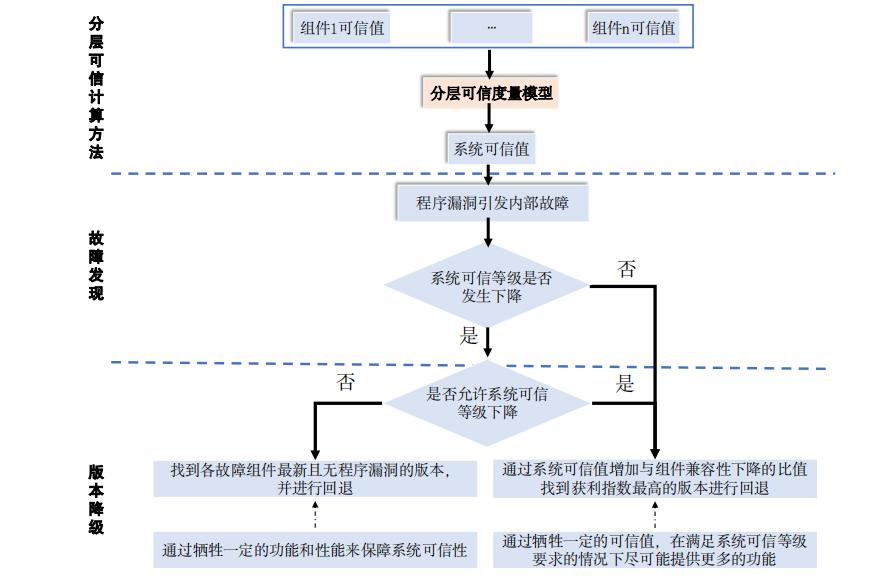
\includegraphics[width=0.8\textwidth]{img10/model.png}
    \caption{优雅降级模型架构}
\end{figure}

优雅降级模型的架构包含以下几个关键部分:

分层结构:系统按照功能模块和组件进行分层,如权限管理、数据更新、数据修改、注册登录、购票下单等功能模块,每层包含若干组件。
每个组件的可信度与其在系统中的调用频率、重要性权重和依赖关系相关。

故障发现机制:通过实时监控系统和组件的可信度,识别系统可信值的下降情况,定位发生故障的组件。

故障隔离机制:通过版本回退或功能降级,将故障组件隔离,以确保其他组件和系统整体的正常运行。
使用算法(如二分搜索算法)快速找到故障组件的最优回退版本,同时尽量降低版本回退对系统兼容性的影响。

版本选择和回退成本控制:使用分支定界法或类似的优化算法,根据组件的重要性权重和回退成本,选择最优的组件版本回退方案,以实现系统可信等级的恢复或保持。

\section{第六题:如何选择组件版本}

可通过基于分层可信度量模型所开发的软件系统分层可信度量工
具对各组件可信度的实时监控,可根据组件可信度的下降情况及下
降原因完成故障组件的定位。

为了保证能在较短时间内找到故障组件
的最优回退版本,可以采用二分搜索算法的思想,通过不断缩小搜索区间
直到找寻到各故障组件的最优回退版本。

\textbf{但如果可信等级已经发生了下降},此时需通过基于分支定界法的故障组件选取算法
来搜寻最优的故障组件选择方案。

核心的公式如下:

\subsection*{(1) 自重要性 \(S(cp)\)}
\textbf{定义:} 衡量单个组件的自身重要性,基于其在系统中被调用的频率。  
公式如下:
\[
S(cp) = \frac{\text{frq}_i}{\sum_{j=1}^n \text{frq}_j} \times 10
\]
其中:
\begin{itemize}
    \item \(\text{frq}_i\): 组件节点 \(cp_i\) 的调用频率。
    \item \(n\): 系统中的组件总数。
\end{itemize}

\subsection*{(2) 出度重要性 \(\text{IMout(cp)}\)}
\textbf{定义:} 根据组件的依赖关系,计算其对其他组件的影响。  
公式如下:
\[
\text{IMout(cp)} = \max \{w_{i,j}\} \times \text{outdegree}
\]
其中:
\begin{itemize}
    \item \(w_{i,j}\): 从 \(cp_i\) 到 \(cp_j\) 的依赖关系的权重。
    \item \(\text{outdegree}\): 组件的出度(依赖关系数量)。
\end{itemize}

\subsection*{(3) 综合重要性 \(IM(cp)\)}
\textbf{定义:} 组件综合重要性指标,结合出度和自重要性。  
公式如下:
\[
IM(cp) = p \times \text{IMout(cp)} + (1-p) \times S(cp)
\]
其中:
\begin{itemize}
    \item \(p\): 权重系数,衡量出度和自重要性的重要性比例。
\end{itemize}

\subsection*{(4) 回退成本 \(Cost(i)\)}
\textbf{公式定义:} 综合考虑组件版本回退的影响,计算其成本:
\[
\text{Cost}(i) = \alpha_i \times \sum_{r_{i,j} \in R_i} \left( \alpha_j \times \frac{\Delta X_i}{X_i} (10 - |X_i - X_j|) + \alpha_j \times \frac{\Delta Y_i}{Y_i} (10 - \beta |Y_i - Y_j|) \right)
\]
其中:
\begin{itemize}
    \item \(\alpha_i\): 组件 \(cp_i\) 的权重。
    \item \(R_i\): 组件 \(cp_i\) 的依赖集合。
    \item \(\Delta X_i = |X_i^* - X_i|\): 主版本号的差值。
    \item \(\Delta Y_i = |Y_i^* - Y_i|\): 次版本号的差值。
    \item \(X_i^*\), \(Y_i^*\): 当前版本的主版本号和次版本号。
    \item \(\beta\): 次版本号权重参数,用于调整次版本号差异的影响。
\end{itemize}

\end{document}
